
\chapter{Structures}

Much of computer science deals with representing and manipulating
information. To do this, people have devised various \textbf{structures}
for organizing chunks of data in a way that makes it easy to store, search,
and retrieve. There's a whole course in most computer science curricula
called ``data structures" which covers how to implement these structures in
code. In this book, we won't be talking about the code, but rather the
abstract structures themselves. This chapter has a lot of pictures in it,
which depict examples of the various structures in a very general way. The
concepts here map directly to code when you need to put them into practice.

\index{data structures}
\index{graphs}
\index{trees}
There are all kinds of data structures --- arrays, linked lists, queues,
stacks, hashtables, and heaps, to name a few --- but they almost all boil
down to one of two fundamental kinds of things: graphs, and trees.  These
are the two structures we'll focus on in this chapter. A graph is just
about the most general structure you can envision: a bunch of scattered
data elements that are related to each other in some way. Almost every data
structure imaginable can be recast as a type of graph. Trees are sort of a
special case of graphs, but also sort of a topic in their own right, kind
of like functions were a special type of relation, but also kind of
different. A tree can be seen as a type of graph that imposes extra special
conditions which give some navigational benefit.

\section{Graphs}

\index{graphs}
\index{vertex/vertices}
\index{edges}
\index{Booth, John Wilkes}
\index{Lincoln, Abraham}
In many ways, the most elegant, simple, and powerful way of representing
knowledge is by means of a \textbf{graph}. A graph is composed of a bunch of
little bits of data, each of which may (or may not) be attached to each of the
others. An example is in Figure~\ref{graph}. Each of the labeled ovals is
called a \textbf{vertex} (plural: \textit{vertices}), and the lines between
them are called \textbf{edges}. Each vertex does, or does not, contain an edge
connecting it to each other vertex. One could imagine each of the vertices
containing various descriptive attributes --- perhaps the \textsl{John Wilkes
Booth} oval would have information about Booth's birthdate, and
\textsl{Washington, DC} information about its longitude, latitude, and
population --- but these are typically not shown on the diagram. All that
really matters, graph-wise, is what vertices it contains, and which ones are
joined to which others.

\begin{figure}[ht]
\centering
\includegraphics[width=0.7\textwidth]{graph.png}
\caption{A graph (undirected).}
\label{graph}
\end{figure}

\index{psychology}
Cognitive psychologists, who study the internal mental processes of the
mind, have long identified this sort of structure as the principal way that
people mentally store and work with information. After all, if you step
back a moment and ask ``what is the `stuff' that's in my memory?" a
reasonable answer is ``well I know about a bunch of things, and the
properties of those things, and the relationships between those things." If
the ``things" are vertices, and the ``properties" are attributes of those
vertices, and the ``relationships" are the edges, we have precisely the
structure of a graph. Psychologists have given this another name: a
\index{semantic network}
\textit{semantic network}. It is thought that the myriad of concepts you
have committed to memory --- \textsl{Abraham Lincoln}, and \textsl{bar of
soap}, and \textsl{my fall schedule}, and perhaps millions of others ---
are all associated in your mind in a vast semantic network that links the
related concepts together. When your mind recalls information, or deduces
facts, or even drifts randomly in idle moments, it's essentially traversing
this graph along the various edges that exist between vertices.

\index{MapQuest}
\index{Facebook}
\index{World Wide Web}
\index{Internet}
That's deep. But you don't have to go near that deep to see the appearance
of graph structures all throughout computer science. What's MapQuest, if
not a giant graph where the vertices are travelable locations and the edges
are routes between them? What's Facebook, if not a giant graph where the
vertices are people and the edges are friendships? What's the World Wide
Web, if not a giant graph where the vertices are pages and the edges are
hyperlinks? What's the Internet, if not a giant graph where the vertices
are computers or routers and the edges are communication links between
them? This simple scheme of linked vertices is powerful enough to
accommodate a whole host of applications, which is why it's worth studying.

\subsection{Graph terms}

The study of graphs brings with it a whole bevy of new terms which are
important to use precisely:

\begin{description}

\index{vertex/vertices}
\index{nodes (of a graph)}
\index{empty graph}
\item[vertex.] Every graph contains zero or more vertices.\footnote{The
phrase ``zero or more" is common in discrete math. In this case, it
indicates that the \textbf{empty graph}, which contains no vertices at all,
is still a legitimate graph.} (These are also sometimes called nodes,
concepts, or objects.)

\index{edges}
\index{links (in a graph)}
\index{loops (in a graph)}
\item[edge.] Every graph contains zero or more edges. (These are also
sometimes called links, connections, associations, or relationships.) Each
edge connects exactly two vertices, unless the edge connects a vertex to
itself, which is possible, believe it or not. An edge that connects a
vertex to itself is called a \textbf{loop}.

\index{paths (in a graph)}
\item[path.] A path is a sequence of consecutive edges that takes you from
one vertex to the other. In Figure~\ref{graph}, there is a path between
\textsl{Washington, DC} and \textsl{John Wilkes Booth} (by means of
\textsl{Ford's Theatre}) even though there is no direct edge between the
two. By contrast, no path exists between \textsl{President} and
\textsl{Civil War}. Don't confuse the two terms edge and path: the former
is a single link between two nodes, while the second can be a whole
step-by-step traversal. (A single edge does count as a path, though.)

\index{directed graphs}
\index{undirected graphs}
\item[directed/undirected.] In some graphs, relationships between nodes are
inherently bidirectional: if $A$ is linked to $B$, then $B$ is linked
to $A$, and it doesn't make sense otherwise. Think of Facebook: friendship
always goes both ways. This kind of graph is called an \textbf{undirected}
graph, and like the Abraham Lincoln example in Figure~\ref{graph}, the
edges are shown as straight lines. In other situations, an edge from $A$ to
$B$ doesn't necessarily imply one in the reverse direction as well. In the
World Wide Web, for instance, just because webpage $A$ has a link on it to
webpage $B$ doesn't mean the reverse is true (it usually isn't). In this
kind of \textbf{directed} graph, we draw arrowheads on the lines to
indicate which way the link goes. An example is Figure~\ref{directedGraph}:
the vertices represent famous boxers, and the directed edges indicate which
boxer defeated which other(s). It is possible for a pair of vertices to
have edges in both directions --- Muhammad Ali and Joe Frazier each
defeated the other (in separate bouts, of course) --- but this is not the
norm, and certainly not the rule, with a directed graph.

\begin{figure}[ht]
\centering
\includegraphics[width=0.7\textwidth]{directedGraph.png}
\caption{A directed graph.}
\label{directedGraph}
\end{figure}

\index{weighted graphs}
\index{weight (of an edge)}
\item[weighted.] Some graphs, in addition to merely containing the
\textit{presence} (or absence) of an edge between each pair of vertices,
also have a number on each edge, called the edge's \textbf{weight}.
Depending on the graph, this can indicate the distance, or cost, between
vertices. An example is in Figure~\ref{weightedGraph}: in true MapQuest
fashion, this graph contains locations, and the mileage between them. A
graph can be both directed and weighted, by the way. If a pair of vertices
in such a graph is attached ``both ways," then each of the two edges will
have its own weight.

\begin{figure}[ht]
\centering
\includegraphics[width=0.6\textwidth]{weightedGraph.png}
\caption{A weighted (and undirected) graph.}
\label{weightedGraph}
\end{figure}

\index{adjacent (vertices)}
\item[adjacent.] If two vertices have an edge between them, they are said
to be adjacent.

\index{connected (vertices/graphs)}
\item[connected.] The word \textbf{connected} has two meanings: it applies
both to pairs of vertices and to entire graphs.

\index{reachable}
We say that two vertices are connected if there is at least one path
between them. Each vertex is therefore ``reachable" from the other.  In
Figure~\ref{graph}, \textsl{President} and \textsl{actor} are connected,
but \textsl{Ford's Theatre} and \textsl{Civil War} are not.

``Connected" is also used to describe entire graphs, if \textit{every}
node can be reached from all others. It's easy to see that
Figure~\ref{weightedGraph} is a connected graph, whereas Figure~\ref{graph}
is not (because \textsl{Civil War} and \textsl{Gettysburg} are isolated
from the other nodes). It's not always trivial to determine whether a graph
is connected, however: imagine a tangled morass of a million vertices, with
ten million edges, and having to figure out whether or not every vertex is
reachable from every other. (And if that seems unrealistically large,
consider Facebook, which has over a billion nodes.)

\index{degree (of a vertex)}
\item[degree.] A vertex's degree is simply the number of edges that connect
to it. \textsl{Virginia Beach} has degree 2, and \textsl{Fredericksburg} 3.
In the case of a directed graph, we sometimes distinguish between the
number of incoming arrows a vertex has (called its \textbf{in-degree}) and
the number of outgoing arrows (the \textbf{out-degree}). \textsl{Muhammad
Ali} had a higher out-degree (3) than in-degree (1) since he won most of
the time.

\index{cycles}
\item[cycle.] A cycle is a path that begins and ends at the same
vertex.\footnote{We'll also say that a cycle can't repeat any edges or
vertices along the way, so that it can't go back and forth repeatedly and
pointlessly between two adjacent nodes. Some mathematicians call this a
\textbf{simple cycle} to distinguish it from the more general
\textbf{cycle}, but we'll just say that no cycles can repeat like this.} In
Figure~\ref{weightedGraph}, \textsl{Richmond}--to--\textsl{Virginia
Beach}--to--\textsl{Fredericksburg}--to--\textsl{Richmond} is a cycle.  Any
loop is a cycle all by itself. For directed graphs, the entire loop must
comprise edges in the ``forward" direction: no fair going backwards. In
Figure~\ref{directedGraph},
\textsl{Frazier}--to--\textsl{Ali}--to--\textsl{Foreman}--to--\textsl{Frazier}
is a cycle, as is the simpler
\textsl{Ali}--to--\textsl{Frazier}--to--\textsl{Ali}.

\index{DAGs (directed acyclic graphs)}
\item[DAG (directed, acyclic graph).] One common use of graphs is to
represent flows of dependencies, for instance the prerequisites that
different college courses have for one another. Another example is project
management workflows: the tasks needed to complete a project become
vertices, and then the dependencies they have on one another become edges.
The graph in Figure~\ref{DAG} shows the steps in making a batch of
brownies, and how these steps depend on each other. The eggs have to be
cracked before the ingredients can be mixed, and the oven has to be
preheated before baking, but the pan can be greased any old time, provided
that it's done before pouring the brown goop into it.

\begin{figure}[ht]
\centering
\includegraphics[width=0.6\textwidth]{DAG.png}
\caption{A DAG.}
\label{DAG}
\end{figure}

\index{directed graphs}
\index{acyclic (graphs)}
A graph of dependencies like this must be both \textbf{directed} and
\textbf{acyclic}, or it wouldn't make sense. Directed, of course, means
that task X can require task Y to be completed before it, without the
reverse also being true. If they both depended on each other, we'd have an
infinite loop, and no brownies could ever get baked! Acyclic means that
\textit{no} kind of cycle can exist in the graph, even one that goes
through multiple vertices. Such a cycle would again result in an infinite
loop, making the project hopeless. Imagine if there were an arrow from
\textsl{bake for 30 mins} back to \textsl{grease pan} in Figure~\ref{DAG}.
Then, we'd have to grease the pan before pouring the goop into it, and we'd
have to pour the goop before baking, but we'd also have to bake before
greasing the pan! We'd be stuck right off the bat: there'd be no way to
complete any of those tasks since they'd all indirectly depend on each
other. A graph that is both directed and acyclic (and therefore free of
these problems) is sometimes called a \textbf{DAG} for short.

\end{description}


\subsection{Spatial positioning}

\index{spatial positioning}
\index{Ali, Muhammad}
\index{Liston, Sonny}
\index{Foreman, George}
\index{Frazier, Joe}
One important thing to understand about graphs is which aspects of a
diagram are relevant. Specifically, \textit{the spatial positioning of the
vertices doesn't matter.} In Figure~\ref{directedGraph} we drew
\textsl{Muhammad Ali} in the mid-upper left, and \textsl{Sonny Liston}  in
the extreme upper right. But this was an arbitrary choice, and irrelevant.
More specifically, this isn't part of the information the diagram claims to
represent. We could have positioned the vertices differently, as in
Figure~\ref{directedGraphDiff}, and had \textit{the same graph}. In both
diagrams, there are the same vertices, and the same edges between them
(check me). Therefore, these are mathematically the same graph.

\begin{figure}[ht]
\centering
\includegraphics[width=0.7\textwidth]{directedGraphDiff.png}
\caption{A different look to \textbf{the same graph as
Figure~\ref{directedGraph}}.}
\label{directedGraphDiff}
\end{figure}

\index{MapQuest}
\index{extensional}
This might not seem surprising for the prize fighter graph, but for graphs
like the MapQuest graph, which actually represent physical locations, it
can seem jarring. In Figure~\ref{weightedGraph} we could have drawn
\textsl{Richmond} north of \textsl{Fredericksburg}, and \textsl{Virginia
Beach} on the far west side of the diagram, and still had the same graph,
provided that all the nodes and links were the same. Just remember that the
spatial positioning is designed for human convenience, and isn't part of
the mathematical information. It's similar to how there's no order to the
elements of a set, even though when we specify a set extensionally, we have
to list them in \textit{some} order to avoid writing all the element names
on top of each other. On a graph diagram, we have to draw each vertex
\textit{somewhere}, but where we put it is simply aesthetic.


\subsection{Relationship to sets}

\index{sets}
\index{Harry Potter}
\index{endorelations}
We seem to have strayed far afield from sets with all this graph stuff. But
actually, there are some important connections to be made to those original
concepts. Recall the wizards set $A$ from chapter~\ref{chap:relations}
that we extended to contain \{~Harry, Ron, Hermione, Neville~\}. Now
consider the following endorelation on $A$:

\begin{center}
(Harry, Ron) \\
(Ron, Harry) \\
(Ron, Hermione) \\
(Ron, Neville) \\
(Hermione, Hermione) \\
(Neville, Harry)
\end{center}

This relation, and all it contains, is represented faithfully by the graph
in Figure~\ref{relationgraph}. The elements of $A$ are the vertices of
course, and each ordered pair of the relation is reflected in an edge of
the graph. Can you see how \textit{exactly} the same information is
represented by both forms?

\begin{figure}[ht]
\centering
\includegraphics[width=0.5\textwidth]{relationGraph.png}
\caption{A graph depicting a endorelation.}
\label{relationgraph}
\end{figure}

\index{undirected graphs}
\index{symmetric (relation)}
Figure~\ref{relationgraph} is a directed graph, of course. What if it were
an undirected graph? The answer is that the corresponding relation would be
\textit{symmetric}. An undirected graph implies that if there's an edge
between two vertices, it goes ``both ways." This is really identical to
saying a relation is symmetric: if an $(x,y)$ is in the relation, then the
corresponding $(y,x)$ must also be. An example is
Figure~\ref{symrelationgraph}, which depicts the following symmetric
relation:

\begin{center}
(Harry, Ron) \\
(Ron, Harry) \\
(Ron, Hermione) \\
(Hermione, Ron) \\
(Harry, Harry) \\
(Neville, Neville)
\end{center}

\begin{figure}[ht]
\centering
\includegraphics[width=0.3\textwidth]{symRelationGraph.png}
\caption{A graph depicting a symmetric endorelation.}
\label{symrelationgraph}
\end{figure}

\index{loops (in a graph)}
Notice how the loops (edges from a node back to itself) in these diagrams
represent ordered pairs in which both elements are the same.

\index{partitions}
Another connection between graphs and sets has to do with partitions.
Figure~\ref{symrelationgraph} was not a connected graph: Neville couldn't
be reached from any of the other nodes. Now consider: isn't a graph like
this similar in some ways to a \textit{partition} of $A$ --- namely, this
one?

\begin{center}
\{~Harry, Ron, Hermione~\} and
\{~Neville~\}.
\end{center}

We've simply partitioned the elements of $A$ into the groups that are
connected. If you remove the edge between Harry and Ron in that graph, you
have:

\begin{center}
\{~Harry~\},
\{~Ron, Hermione~\}, and
\{~Neville~\}.
\end{center}

Then add one between Hermione and Neville, and now you have:

\begin{center}
\{~Harry~\} and
\{~Ron, Hermione, Neville~\}.
\end{center}

\index{connected (vertices/graphs)}
In other words, the ``connectedness" of a graph can be represented
precisely as a partition of the set of vertices. Each connected subset is
in its own group, and every vertex is in one and only one group: therefore,
these isolated groups are mutually exclusive and collectively exhaustive.
Cool.

\subsection{Graph traversal}

If you had a long list --- perhaps of phone numbers, names, or purchase
orders --- and you needed to go through and do something to each element of
the list --- dial all the numbers, scan the list for a certain name, add up
all the orders --- it'd be pretty obvious how to do it. You just start at
the top and work your way down. It might be tedious, but it's not
confusing.

\index{traversal}
Iterating through the elements like this is called \textbf{traversing} the
data structure. You want to make sure you encounter each element once (and
only once) so you can do whatever needs to be done with it. It's clear how
to traverse a list. But how to traverse a graph? There is no obvious
``first" or ``last" node, and each one is linked to potentially many
others. And as we've seen, the vertices might not even \textit{be} fully
connected, so a traversal path through all the nodes might not even exist.

There are two different ways of traversing a graph: breadth-first, and
depth-first. They provide different ways of exploring the nodes, and as a
side effect, each is able to discover whether the graph is connected or
not. Let's look at each in turn.

\subsubsection{Breadth-first traversal}
\index{BFT (breadth-first traversal)}

With \textbf{breadth-first traversal}, we begin at a starting vertex (it
doesn't matter which one) and explore the graph cautiously and delicately.
We probe equally deep in all directions, making sure we've looked a little
ways down each possible path before exploring each of those paths a little
further.

\index{queue}
\index{enqueueing}
\index{dequeueing}
\index{FIFO}
To do this, we use a very simple data structure called a \textbf{queue}. A
queue is simply a list of nodes that are waiting in line. (In Britain, I'm
told, instead of saying ``line up" at the sandwich shop, they say ``queue
up.") When we enter a node into the queue at the tail end, we call it
\textbf{enqueueing} the node, and when we remove one from the front, we
call it \textbf{dequeueing} the node. The nodes in the middle patiently
wait their turn to be dealt with, getting closer to the front every time
the front node is dequeued. 

An example of this data structure in action is shown in Figure~\ref{queue}.
Note carefully that we always insert nodes at one end (on the right) and
remove them from the \textit{other} end (the left). This means that the
first item to be enqueued (in this case, the triangle) will be the first to
be dequeued. ``Calls will be answered in the order they were received."
This fact has given rise to another name for a queue: a ``\textbf{FIFO},"
which stands for ``first-in-first-out."

\afterpage{\clearpage}

\begin{figure}[ht]
\centering
\begin{tabular}{l l}
\textit{Start with an empty queue:} & $|$ \\
\hline
\textit{Enqueue a triangle, and we have:} & $|\triangle$ \\
\hline
\textit{Enqueue a star, and we have:} & $|\triangle \bigstar$ \\
\hline
\textit{Enqueue a heart, and we have:} & $|\triangle \bigstar \heartsuit$ \\
\hline
\textit{Dequeue the triangle, and we have:} & $|\bigstar \heartsuit$ \\
\hline
\textit{Enqueue a club, and we have:} & $|\bigstar \heartsuit \clubsuit$ \\
\hline
\textit{Dequeue the star, and we have:} & $|\heartsuit \clubsuit$ \\
\hline
\textit{Dequeue the heart, and we have:} & $|\clubsuit$ \\
\hline
\textit{Dequeue the club. We're empty again:} & $|$ \\
\end{tabular}
\caption{A queue in action. The vertical bar marks the ``front of the
line," and the elements are waiting to be dequeued in order from left to
right.}
\label{queue}
\end{figure}

Now here's how we use a queue to traverse a graph breadth-first. We're
going to start at a particular node, and put all of its adjacent nodes into
a queue. This makes them all safely ``wait in line" until we get around to
exploring them. Then, we repeatedly take the first node in line, do
whatever we need to do with it, and then put all of \textit{its} adjacent
nodes in line. We keep doing this until the queue is empty.

\index{marking (a node)}
Now it might have occurred to you that we can run into trouble if we
encounter the same node multiple times while we're traversing. This can
happen if the graph has a cycle: there will be more than one path to reach
some nodes, and we could get stuck in an infinite loop if we're not
careful. For this reason, we introduce the concept of \textbf{marking} 
nodes. This is kind of like leaving a trail of breadcrumbs: if we're ever
about to explore a node, but find out it's marked, then we know we've
already been there, and it's pointless to search it again.

So there are two things we're going to do to nodes as we search:

\index{visiting (a node)}
\begin{itemize} 
\item To \textbf{mark} a node means to remember that we've already
encountered it in the process of our search.
\item To \textbf{visit} a node means to actually do whatever it is we need
to do to the node (call the phone number, examine its name for a pattern
match, add the number to our total, whatever.)
\end{itemize} 

\index{algorithm}
Now then. Breadth-first traversal (BFT) is an \textbf{algorithm}, which is
just a step-by-step, reliable procedure that's guaranteed to produce a
result. In this case, it's guaranteed to visit every node in the graph
that's reachable from the starting node, and not get stuck in any infinite
loops in the process. Here it is:

\index{BFT (breadth-first traversal)}
\vspace{.1in}
\begin{framed}
\textbf{Breadth-first traversal (BFT)}
\begin{compactenum}
\itemsep.1em
\item Choose a starting node.
\item Mark it and enqueue it on an empty queue.
\item While the queue is not empty, do these steps:
    \begin{compactenum}
    \item Dequeue the front node of the queue.
    \item Visit it.
    \item Mark and enqueue all of its \textit{unmarked} adjacent nodes (in
any order).
    \end{compactenum}
\end{compactenum}
\end{framed}
\vspace{.2in}

\index{Facebook}
\index{queue}
Let's run this algorithm in action on a set of Facebook users. 
Figure~\ref{BFT} depicts eleven users, and the friendships between them.
First, we choose Greg as the starting node (not for any particular reason,
just that we have to start somewhere). We mark him (in grey on the diagram)
and put him in the queue (the queue contents are listed at the bottom of
each frame, with the front of the queue on the left). Then, we begin our
loop. When we take Greg off the queue, we visit him (which means we ``do
whatever we need to do to Greg") and then mark and enqueue his adjacent
nodes Chuck and Izzy. It does not matter which order we put them into the
queue, just as it did not matter what node we started with. In pane 3,
Chuck has been dequeued, visited, and \textit{his} adjacent nodes put on
the queue. Only one node gets enqueued here --- Adrian --- because
obviously Greg has already been marked (and even visited, no less) and this
marking allows us to be smart and not re-enqueue him.

It's at this point that the ``breadth-first" feature becomes apparent.
We've just finished with Chuck, but instead of exploring Adrian next,
\textit{we resume with Izzy.} This is because she has been waiting
patiently on the queue, and her turn has come up. So we lay Adrian aside
(in the queue, of course) and visit Izzy, enqueueing her neighbor Elaine in
the process. \textit{Then}, we go back to Adrian. The process continues, in
``one step on the top path, one step on the bottom path" fashion, until our
two exploration paths actually meet each other on the back end. Visiting
Jackie causes us to enqueue Brittany, and then when we take Kim off the
queue, we do not re-enqueue Brittany because she has been marked and so we
know she's already being taken care of. 

For space considerations, Figure~\ref{BFT} leaves off at this point, but of
course we would continue visiting nodes in the queue until the queue was
empty. As you can see, Hank and Danielle will not be visited at all in this
process: this is because apparently nobody they know knows anybody in the
Greg crowd, and so there's no way to reach them from Greg. This is what I
meant earlier by saying that as a side effect, the BFT algorithm tells us
whether the graph is connected or not. All we have to do is start
somewhere, run BFT, and then see whether any nodes have not been marked and
visited. If there are any, we can continue with another starting point, and
then repeat the process.


\begin{figure}[ht]
\centering
\begin{custommargins}{-1.4cm}{-1.8cm}
\framebox{\includegraphics[width=0.32\textwidth]{BFT1.png}}
\framebox{\includegraphics[width=0.32\textwidth]{BFT2.png}}
\framebox{\includegraphics[width=0.32\textwidth]{BFT3.png}}
\framebox{\includegraphics[width=0.32\textwidth]{BFT4.png}}
\framebox{\includegraphics[width=0.32\textwidth]{BFT5.png}}
\framebox{\includegraphics[width=0.32\textwidth]{BFT6.png}}
\framebox{\includegraphics[width=0.32\textwidth]{BFT7.png}}
\framebox{\includegraphics[width=0.32\textwidth]{BFT8.png}}
\framebox{\includegraphics[width=0.32\textwidth]{BFT9.png}}
\caption{The stages of breadth-first traversal. Marked nodes are grey, and
visited nodes are black. The order of visitation is: G, C, I, A, E, J, K,
F, B.}
\label{BFT}
\end{custommargins}
\end{figure}

\afterpage{\clearpage}

\subsubsection{Depth-first traversal (DFT)}
\index{DFT (depth-first traversal)}

With \textbf{depth-first traversal}, we explore the graph boldly and
recklessly. We choose the first direction we see, and plunge down it all
the way to its depths, before reluctantly backing out and trying the other
paths from the start. 

\newcommand{\stackcell}[2][c]{%
  \begin{tabular}[#1]{@{}c@{}}#2\end{tabular}}
 
\index{stack}
\index{top (of a stack)}
\index{push (on a stack)}
\index{pop (off a stack)}
The algorithm is almost identical to BFT, except that instead of a queue,
we use a \textbf{stack}. A stack is the same as a queue except that
instead of putting elements on one end and taking them off the other, you
\textit{add and remove to the same end.} This ``end" is called the
\textbf{top} of the stack. When we add an element to this end, we say we
\textbf{push} it on the stack, and when we remove the top element, we say
we \textbf{pop} it off.

\begin{figure}
\centering
\begin{tabular}{l l}
\textit{Start with an empty stack:} & $\underline{\quad}$ \\
\hline
\textit{Push a triangle, and we have:} & $\underline{\triangle}$ \\
\hline
\textit{Push a star, and we have:} & \stackcell{$\bigstar$ \\ $\underline{\triangle}$} \\
\hline
\textit{Push a heart, and we have:} & \stackcell{$\heartsuit$ \\ $\bigstar$ \\ $\underline{\triangle}$} \\
\hline
\textit{Pop the heart, and we have:} & \stackcell{$\bigstar$ \\ $\underline{\triangle}$} \\
\hline
\textit{Push a club, and we have:} & \stackcell{$\clubsuit$ \\ $\bigstar$ \\ $\underline{\triangle}$} \\
\hline
\textit{Pop the club, and we have:} & \stackcell{$\bigstar$ \\ $\underline{\triangle}$} \\
\hline
\textit{Pop the star, and we have:} & $\underline{\triangle}$ \\
\hline
\textit{Pop the triangle. We're empty again:} & $\underline{\quad}$
\end{tabular}
\caption{A stack in action. The horizontal bar marks the bottom of the
stack, and the elements are pushed and popped from the top.}
\label{stack}
\end{figure}

\index{LIFO}
You can think of a stack as...well, a stack, whether of books or cafeteria
trays or anything else. You can't get anything out of the middle of a
stack, but you can take items off and put more items on. Figure~\ref{stack}
has an example. The first item pushed is always the last one to be popped,
and the most recent one pushed is always ready to be popped back off, and
so a stack is also sometimes called a ``\textbf{LIFO}" (last-in-first-out.)


The depth-first traversal algorithm itself looks like d\'ej\`a vu all over
again. All you do is replace ``queue" with ``stack":

\index{DFT (depth-first traversal)}
\vspace{.1in}
\begin{samepage}
\begin{framed}
\textbf{Depth-first traversal (DFT)}
\begin{compactenum}
\item Choose a starting node.
\item Mark it and push it on an empty stack.
\item While the stack is not empty, do these steps:
    \begin{compactenum}
    \item Pop the top node off the stack.
    \item Visit it.
    \item Mark and push all of its \textit{unmarked} adjacent nodes (in
any order).
    \end{compactenum}
\end{compactenum}
\end{framed}
\end{samepage}
\vspace{.2in}

\index{stack}
The algorithm in action is shown in Figure~\ref{DFT}. The stack really made
a difference! Instead of alternately exploring Chuck's and Izzy's paths, it
bullheadedly darts down Chuck's path as far as it can go, all the way to
hitting Izzy's back door. Only then does it back out and visit Izzy. This
is because the stack always pops off what it just pushed on, whereas
whatever got pushed first has to wait until everything else is done before
it gets its chance. That first couple of pushes was critical: if we had
pushed Chuck before Izzy at the very beginning, then we would have explored
\textit{Izzy's} entire world before arriving at Chuck's back door, instead
of the other way around. As it is, Izzy got put on the bottom, and so she
stayed on the bottom, which is inevitable with a stack.

DFT identifies disconnected graphs in the same way as BFT, and it similarly
avoids getting stuck in infinite loops when it encounters cycles. The only
difference is the order in which it visits the nodes.

\afterpage{\clearpage}

\begin{figure}[ht]
\centering
\begin{custommargins}{-1.4cm}{-1.8cm}
\framebox{\includegraphics[width=0.32\textwidth]{DFT1.png}}
\framebox{\includegraphics[width=0.32\textwidth]{DFT2.png}}
\framebox{\includegraphics[width=0.32\textwidth]{DFT3.png}}
\framebox{\includegraphics[width=0.32\textwidth]{DFT4.png}}
\framebox{\includegraphics[width=0.32\textwidth]{DFT5.png}}
\framebox{\includegraphics[width=0.32\textwidth]{DFT6.png}}
\framebox{\includegraphics[width=0.32\textwidth]{DFT7.png}}
\framebox{\includegraphics[width=0.32\textwidth]{DFT8.png}}
\framebox{\includegraphics[width=0.32\textwidth]{DFT9.png}}

\caption{The stages of depth-first traversal. Marked nodes are grey, and
visited nodes are black. The order of visitation is: G, C, A, J, B, K, F,
E, I.}
\label{DFT}
\end{custommargins}
\end{figure}

\subsection{Finding the shortest path}

\index{Dijkstra, Edsger}
\index{Dijkstra's algorithm}
\index{weighted graphs}
We'll look at two other important algorithms that involve graphs,
specifically \textit{weighted} graphs. The first one is called
\textbf{Dijkstra's shortest-path algorithm.} This is a procedure for
finding the shortest path between two nodes, if one exists. It was invented
in 1956 by the legendary computer science pioneer Edsger Dijkstra, and is
widely used today by, among other things, network routing protocols.

\index{France}
\index{World War II}
Consider Figure~\ref{france}, a simplified map of France circa November
1944. Fresh U.S. troops are arriving by ship at the port town of Bordeaux,
and need to reach Strasbourg as quickly as possible to assist the Allies in
pushing Nazi squadrons back into Germany. The vertices of this graph are
French cities, and the edge weights represent marching distances in
kilometers. Although D-Day was successful, the outcome of the War may
depend on how quickly these reinforcements can reach the front.

\begin{figure}[ht]
\centering
\includegraphics[width=0.6\textwidth]{DijkstraOrig.png}
\caption{A weighted graph, through which we desire to find the shortest
path from Bordeaux to Strasbourg.}
\label{france}
\end{figure}

The question, obviously, is which path the troops should take so as to
reach Strasbourg the soonest. With a graph this small, you might be able to
eyeball it. (Try it!) But Dijksta's algorithm systematically considers
every possible path, and is guaranteed to find the one with the shortest
total distance.

\index{tentative best distance}
The way it works is to assign each node a \textit{tentative} lowest
distance, along with a tentative path from the start node to it. Then, if
the algorithm encounters a different path to the same node as it
progresses, it updates this tentative distance with the new, lower
distance, and replaces the ``best path to it" with the new one. Dijkstra's
algorithm finds the shortest distance from the start node to the end node,
but as a bonus, it actually finds the shortest distance from the start node
to \textit{every} node as it goes. Thus you are left with the best possible
path from your start node to every other node in the graph.

Here's the algorithm in full:

\index{Dijkstra's algorithm}
\index{visiting (a node)}
\index{marking (a node)}
\index{current node}
\vspace{.1in}
\begin{samepage}
\begin{framed}
\textbf{Dijkstra's shortest-path algorithm}
\begin{compactenum}
\item Choose a starting node and an ending node.
\item Mark the tentative distance for the starting node as 0, and all
other nodes as $\infty$.
\item While there are still unvisited nodes, do these steps:
    \begin{compactenum}
    \item \label{choose} Identify the \textit{un}visited node with the smallest tentative
distance. (If this is $\infty$, then we're done. All other nodes are
unreachable.) Call this node the ``current node."
    \item For each unvisited neighbor of the current node, do these steps:
        \begin{compactenum}
        \item Compute the sum of the current node's tentative distance and
the distance from the current node to its neighbor.
        \item Compare this total to the neighbor's current tentative
distance. If it's less than the current tentative distance, update the
tentative distance with this new value, and mark an arrow on the path from
the current node to the neighbor (erasing any other arrow to the neighbor.)
        \item Mark the current node as visited. (Its distance and best path
are now fixed.)
        \end{compactenum}
    \end{compactenum}
\end{compactenum}
\end{framed}
\end{samepage}
\vspace{.2in}

Don't worry, this isn't as hard as it sounds. But you do have to have your
wits about you and carefully update all the numbers. Let's see it in action
for WWII France. In the first frame of Figure~\ref{fig:dijkstra}, we've marked
each node with a diamond containing the tentative shortest distance to it
from Bordeaux. This is 0 for Bordeaux itself (since it's 0 kilometers away
from itself, duh), and infinity for all the others, since we haven't
explored anything yet, and we want to start off as pessimistic as possible.
We'll update these distances to lower values as we find paths to them.

We start with Bordeaux as the ``current node," marked in grey. In frame 2,
we update the best-possible-path and the distance-of-that-path for each of
Bordeaux's neighbors. Nantes, we discover, is no longer ``infinity away,"
but a mere 150 km away, since there is a direct path to it from Bordeaux.
Vichy and Toulouse are similarly updated. Note the heavy arrowed lines on
the diagram, showing the best path (so far) to each of these cities from
Bordeaux. 

Step~\ref{choose} tells us to choose the node with the lowest tentative
distance as the next current node. So for frame 3, Nantes fits the bill
with a (tentative) distance of 150 km. It has only one unmarked neighbor,
Paris, which we update with \textit{450} km. Why 450? Because it took us
150 to get from the start to Nantes, and another 300 from Nantes to Paris.
After updating Paris, Nantes is now set in stone --- we know we'll never
encounter a better route to it than from Bordeaux directly.

Frame 4 is our first time encountering a node that already has a
non-infinite tentative distance. In this case, we \textit{don't} further
update it, because our new opportunity (Bordeaux--to--Toulouse--to--Vichy)
is 500 km, which is longer than going from Bordeaux to Toulouse direct.
Lyon and Marseille are updated as normal.

We now have two unmarked nodes that tie for shortest tentative distance:
Paris, and Vichy (450 km each). In this case, it doesn't matter which we
choose. We'll pick Vichy for no particular reason. Frame 5 then shows some
interesting activity. We do not update the path to Paris, since it would be
800 km through Vichy, whereas Paris already had a much better 450 km path.
Lille is updated from infinity to 850 km, since we found our first path to
it. But Lyon is the really interesting case. It already had a path ---
Bordeaux--to--Toulouse--to--Lyon --- but that path was 800 km, and we have
just found a \textit{better} path: Bordeaux--to--Vichy--to--Lyon, which
only costs 450 + 250 = 700. This means we remove the arrow from Toulouse to
Lyon and draw a new arrow from Vichy to Lyon. Note that the arrow from
Bordeaux to Toulouse doesn't disappear, even though it was part of this
apparently-not-so-great path to Lyon. That's because the best route to
\textit{Toulouse} still \textit{is} along that edge. Just because we
wouldn't use it to go to Lyon doesn't mean we don't want it if we were
going simply to Toulouse.

In frame 6, we take up the other 450 node (Paris) which we temporarily
neglected when we randomly chose to continue with Vichy first. When we do,
we discover a better path to Lille than we had before, and so we update its
distance (to 800 km) and its path (through Nantes and Paris instead of
through Vichy) accordingly.

When we consider Marseille in frame 7, we find another better path: this
time to Lyon. Forget that through--Vichy stuff; it turns out to be a bit
faster to go through Toulouse and Marseille. In other news, we found a way
to Nice.

Hopefully you get the pattern. We continue selecting the unmarked node with
the lowest tentative distance, updating its neighbors' distances and paths,
then marking it ``visited," until we're done with all the nodes. The last
frame shows the completed version (with all nodes colored white again so
you can read them). The verdict is: our troops should go from Bordeaux
through Toulouse, Marseille, Lyon, and Brian\c{c}on on their way to the
fighting in Strasborg, for a total of 1,250 kilometers. Who knew? All other
paths are longer. Note also how in the figure, the shortest distance to
\textit{every} node is easily identified by looking at the heavy arrowed
lines.


\begin{figure}[ht]
\centering
\begin{custommargins}{-2.4cm}{-2.8cm}
\framebox{\includegraphics[width=0.5\textwidth]{Dijkstra1.png}}
\framebox{\includegraphics[width=0.5\textwidth]{Dijkstra2.png}}
\framebox{\includegraphics[width=0.5\textwidth]{Dijkstra3.png}}
\framebox{\includegraphics[width=0.5\textwidth]{Dijkstra4.png}}
\framebox{\includegraphics[width=0.5\textwidth]{Dijkstra5.png}}
\framebox{\includegraphics[width=0.5\textwidth]{Dijkstra6.png}}
\framebox{\includegraphics[width=0.5\textwidth]{Dijkstra7.png}}
\framebox{\includegraphics[width=0.5\textwidth]{Dijkstra8.png}}

\caption{The stages of Dijkstra's shortest-path algorithm. The ``current
node" is shown in grey, with visited nodes (whose best paths and shortest
distances have been unalterably determined) in black. The diamond next to
each node shows the tentative shortest distance to that node from
Bordeaux.}
\label{fig:dijkstra}
\end{custommargins}
\end{figure}

\subsection{Finding the minimal connecting edge set}

So we've figured out the shortest path for our troops. But our field
generals might also want to do something different: establish supply lines.
A supply line is a safe route over which food, fuel, and machinery can be
delivered, with smooth travel and protection from ambush. Now we have
military divisions stationed in each of the eleven French cities, and so
the cities must all be connected to each other via secure paths.
Safeguarding each mile of a supply line takes resources, though, so we want
to do this in the minimal possible way. How can we get all the cities
connected to each other so we can safely deliver supplies between any of
them, using the least possible amount of road?

This isn't just a military problem. The same issue came up in ancient Rome
when aqueducts had to reach multiple cities. More recently, supplying
neighborhoods and homes with power, or networking multiple computers with
Ethernet cable, involves the same question. In all these cases, we're not
after the shortest route between two points. Instead, we're sort of after
the shortest route ``between all the points." We don't care how each pair
of nodes is connected, provided that they \textit{are} connected. And it's
the total length of the required connections that we want to minimize.

\index{Prim's algorithm}
\index{Prim, Robert}
\index{Jarnik, Vojtech}
To find this, we'll use \textbf{Prim's algorithm}, a technique named for
the somewhat obscure computer scientist Robert Prim who developed it in
1957, although it had already been discovered much earlier (1930, by the
Czech mathematician Vojtech Jarnik). Prim's algorithm turns out to be much
easier to carry out than Dijkstra's algorithm, which I find surprising,
since it seems to be solving a problem that's just as hard. But here's all
you do:

\vspace{.1in}
\begin{samepage}
\begin{framed}
\textbf{Prim's minimal connecting edge set algorithm}
\begin{compactenum}
\item Choose a node, any node.
\item While not all the nodes are connected, do these steps:
    \begin{compactenum}
    \item \label{greedystep} Identify the node closest to the 
already-connected nodes, and connect it to those nodes via the shortest
edge.
    \end{compactenum}
\end{compactenum}
\end{framed}
\end{samepage}

\index{greedy algorithm}
That's it. Prim's algorithm is an example of a \textbf{greedy algorithm},
which means that it always chooses the immediately obvious short-term best
choice available. Non-greedy algorithms can say, ``although doing X would
give the highest short-term satisfaction, I can look ahead and see that
choosing Y instead will lead to a better overall result in the long run."
Greedy algorithms, by contrast, always gobble up what seems best at the
time. That's what Prim's algorithm is doing in step~\ref{greedystep}. It
looks for the non-connected node that's immediately closest to the
connected group, and adds it without a second thought. There's no notion of
``perhaps I'll get a shorter overall edge set if I forego connecting this
temptingly close node right now."

Sometimes, a greedy algorithm turns out to give an optimal result. Often it
does not, and more sophisticated approaches can find better solutions.  In
this case, it happens to work out that the greedy approach does work!
Prim's algorithm will always find the set of edges that connects all the
nodes and does so with the lowest possible total distance. It's amazing
that it can do so, especially since it never backtracks or revises its
opinion the way Dijkstra's algorithm does.

Let's follow the algorithm's progress in the WWII example. We can start
with any node, so we'll pick Vichy just at random. Frame 1 of
Figure~\ref{prim} shows what happens when the algorithm begins with Vichy:
we simply examine all its neighbors, and connect the one that's closest to
it. Nothing could be simpler. In this case, Lyon is a mere 250 km away,
which is closer than anything else is to Vichy, so we connect it and add
the Vichy--Lyon edge to our edge set. The figure shows a heavy black line
between Vichy and Lyon to show that it will officially be a supply line.

\begin{figure}[ht]
\centering
\begin{custommargins}{-2.4cm}{-2.8cm}
\framebox{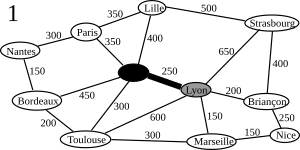
\includegraphics[width=0.5\textwidth]{Prim1.png}}
\framebox{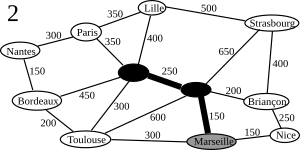
\includegraphics[width=0.5\textwidth]{Prim2.png}}
\framebox{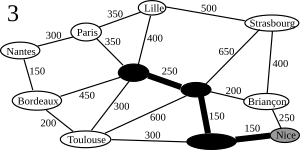
\includegraphics[width=0.5\textwidth]{Prim3.png}}
\framebox{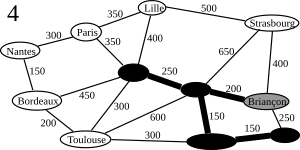
\includegraphics[width=0.5\textwidth]{Prim4.png}}
\framebox{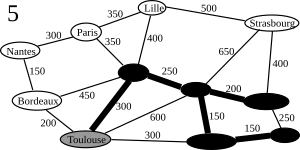
\includegraphics[width=0.5\textwidth]{Prim5.png}}
\framebox{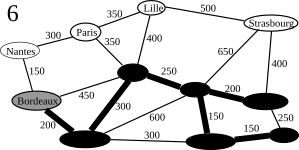
\includegraphics[width=0.5\textwidth]{Prim6.png}}
\framebox{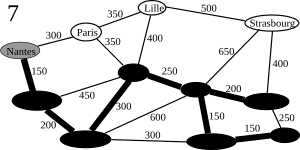
\includegraphics[width=0.5\textwidth]{Prim7.png}}
\framebox{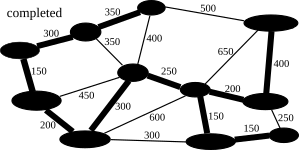
\includegraphics[width=0.5\textwidth]{Prim8.png}}

\caption{The stages of Prim's minimal connecting edge set algorithm. Heavy
lines indicate edges that have been (irrevocably) added to the set.}
\label{prim}
\end{custommargins}
\end{figure}

\afterpage{\clearpage}

And so it goes. In successive frames, we add Marseille, Nice, and Brian\c{c}on
to the set of connected nodes, since we can do no better than 150 km, 150 km,
and 200 km, respectively. Note carefully that in frame 4 we connect
Brian\c{c}on to Lyon -- \textit{not} to Nice -- because $200 <
250$.\footnote{It's very easy to fall into a trance and always add nodes only
to the ends of the growing snake. In fact, I originally did that with this very
example!} Note also that
the algorithm can jump around from side to side --- we aren't looking for the
shortest edge from the most recently added node, but from \textit{any}
connected node.

The final result is shown in the last frame. This is the best way to connect
all the cities to each other, if ``best" means ``least total supply line
distance," which in this case works out to 2450 total kilometers. But if you
look carefully, you'll notice a fascinating thing. \textit{This network of
edges does \textbf{not} contain the shortest path from Bordeaux to Strasbourg!}
I find that result dumbfounding. Wouldn't you think that the shortest path
between any two nodes would land right on this Prim network? Yet if you compare
Figure~\ref{prim} with Figure~\ref{fig:dijkstra} you'll see that the quickest
way from Bordeaux to Strasbourg is through Marseille, not Vichy.

So we end up with the remarkable fact that the shortest route between two
points has nothing whatsoever to do with the shortest \textit{total}
distance between \textit{all} points. Who knew?






\section{Trees}

\index{trees}
A tree is really nothing but a simplification of a graph. There are two
kinds of trees in the world: free trees, and rooted trees.\footnote{There
appears to be no consensus as to which of these concepts is the most basic.
Some authors refer to a free tree simply as a ``tree" --- as though this
were the ``normal" kind of tree --- and use the term rooted tree for the
other kind. Other authors do the opposite. To avoid confusion, I'll try to
always use the full term (although I admit I'm one who considers rooted
trees to be the more important, default concept).}

\subsection{Free trees}

\index{free trees}
A \textbf{free tree} is just a connected graph with no cycles. Every node
is reachable from the others, and there's only one way to get anywhere.
Take a look at Figure~\ref{freetree}. It looks just like a graph (and it
is) but unlike the WWII France graph, it's more skeletal. This is because
in some sense, a free tree doesn't contain anything ``extra."

\begin{figure}[ht]
\centering
\begin{custommargins}{-2.1cm}{-3cm}
\includegraphics[width=0.5\textwidth]{freeTree.png}
\caption{A free tree.}
\label{freetree}
\end{custommargins}
\end{figure}

If you have a free tree, the following interesting facts are true:

\begin{compactenum}
\item There's exactly one path between any two nodes. (Check it!)
\item If you remove any edge, the graph becomes disconnected. (Try it!)
\item If you add any new edge, you end up adding a cycle. (Try it!)
\item \label{onelessedge} If there are $n$ nodes, there are $n-1$ edges. (Think about it!)
\end{compactenum}

So basically, if your goal is connecting all the nodes, and you have a free
tree, you're all set. Adding anything is redundant, and taking away
anything breaks it.

If this reminds you of Prim's algorithm, it should. Prim's algorithm
produced exactly this: a \textit{free tree} connecting all the nodes ---
and specifically the free tree with shortest possible total length. Go back
and look at the final frame of Figure~\ref{prim} and convince yourself that
the darkened edges form a free tree.

\index{Prim's algorithm}
\index{minimal spanning tree}
For this reason, the algorithm is often called \textbf{Prim's minimal
spanning tree algorithm}. A ``spanning tree" just means ``a free tree that
spans (connects) all the graph's nodes." 

Keep in mind that there are many free trees one can make with the same set
of vertices. For instance, if you remove the edge from A to F, and add one
from anything else to F, you have a different free tree.

\subsection{Rooted trees}

\index{trees}
\index{rooted trees}
\index{root (of a tree)}
Now a \textbf{rooted tree} is the same thing as a free tree, except that we
elevate one node to become the \textbf{root}. It turns out this makes all
the difference. Suppose we chose A as the root of Figure~\ref{freetree}.
Then we would have the rooted tree in the left half of
Figure~\ref{rootedtree}. The A vertex has been positioned at the top, and
everything else is flowing under it. I think of it as reaching into the
free tree, carefully grasping a node, and then lifting up your hand so the
rest of the free tree dangles from there. Had we chosen (say) C as the root
instead, we would have a different rooted tree, depicted in the right half
of the figure. Both of these rooted trees have all the same edges as the
free tree did: B is connected to both A and C, F is connected only to A,
\textit{etc.} The only difference is which node is designated the root.

\begin{figure}[ht]
\centering
\begin{custommargins}{-2.1cm}{-3cm}
\includegraphics[width=0.4\textwidth]{rootedTree1.png} \quad\quad\quad
\includegraphics[width=0.35\textwidth]{rootedTree2.png}
\caption{Two different rooted trees with the same vertices and edges.}
\label{rootedtree}
\end{custommargins}
\label{page:rootedtree}
\end{figure}

\index{spatial positioning}
Up to now we've said that the spatial positioning on graphs is irrelevant.
But this changes a bit with rooted trees. Vertical positioning is our only
way of showing which nodes are ``above" others, and the word ``above" does
indeed have meaning here: it means closer to the root. The altitude of a
node shows how many steps it is away from the root. In the right rooted
tree, nodes B, D, and E are all one step away from the root (C), while node
F is three steps away.

\index{paths (in a graph)}
The key aspect to rooted trees --- which is both their greatest advantage
and greatest limitation --- is that \textit{every node has one and only one
path to the root.} This behavior is inherited from free trees: as we noted,
every node has only one path to every other.

\index{filesystems}
Trees have a myriad of applications. Think of the files and folders on your
hard drive: at the top is the root of the filesystem (perhaps ``\texttt{/}"
on Linux/Mac or ``\texttt{C:}\textbackslash\textbackslash" on Windows) and
underneath that are named folders. Each folder can contain files as well as
other named folders, and so on down the hierarchy. The result is that each
file has one, and only one, distinct path to it from the top of the
filesystem.  The file can be stored, and later retrieved, in exactly one
way.

\index{org charts}
An ``org chart" is like this: the CEO is at the top, then underneath her
are the VP's, the Directors, the Managers, and finally the rank-and-file
employees. So is a military organization: the Commander in Chief directs
generals, who command colonels, who command majors, who command captains,
who command lieutenants, who command sergeants, who command privates.

\index{human body}
The human body is even a rooted tree of sorts: it contains skeletal,
cardiovascular, digestive, and other systems, each of which is comprised of
organs, then tissues, then cells, molecules, and atoms. In fact, anything
that has this sort of part-whole containment hierarchy is just asking to be
represented as a tree.

\index{compilers}
\index{HTML}
\index{chess}
\index{object-oriented design}
In computer programming, the applications are too numerous to name.
Compilers scan code and build a ``parse tree" of its underlying meaning.
HTML is a way of structuring plain text into a tree-like hierarchy of
displayable elements. AI chess programs build trees representing their
possible future moves and their opponent's probable responses, in order to
``see many moves ahead" and evaluate their best options. Object-oriented
designs involve ``inheritance hierarchies" of classes, each one specialized
from a specific other. \textit{Etc.} Other than a simple sequence (like an
array), trees are probably the most common data structure in all of
computer science.

\subsubsection{Rooted tree terminology}

\index{rooted trees}
Rooted trees carry with them a number of terms. I'll use the tree on the
left side of Figure~\ref{rootedtree} as an illustration of each:

\begin{description}
\index{root (of a tree)}
\item[root.] The node at the top of the tree, which is A in our example.
Note that unlike trees in the real world, computer science trees have their
root at the top and grow down. Every tree has a root except the
\textbf{empty tree}, which is the ``tree" that has no nodes at all in it.
(It's kind of weird thinking of ``nothing" as a tree, but it's kind of like
the empty set $\varnothing$, which is still a set.) \index{empty set}

\index{parent (of a node)}
\item[parent.] Every node except the root has one parent: the node
immediately above it. D's parent is C, C's parent is B, F's parent is A,
and A has no parent.

\index{child (of a node)}
\item[child.] Some nodes have children, which are nodes connected directly
below it. A's children are F and B, C's are D and E, B's only child is C,
and E has no children.

\index{sibling (of a node)}
\item[sibling.] A node with the same parent. E's sibling is D, B's is F,
and none of the other nodes have siblings.

\index{ancestor (of a node)}
\item[ancestor.] Your parent, grandparent, great-grandparent,
\textit{etc.}, all the way back to the root. B's only ancestor is A, while
E's ancestors are C, B, and A. Note that F is \textit{not} C's ancestor,
even though it's above it on the diagram: there's no connection from C to
F, except back through the root (which doesn't count).

\index{descendant (of a node)}
\item[descendant.] Your children, grandchildren, great-grandchildren,
\textit{etc.}, all the way to the leaves. B's descendants are C, D and E,
while A's are F, B, C, D, and E. 

\index{leaves}
\item[leaf.] A node with no children. F, D, and E are leaves. Note that in
a (very) small tree, the root could itself be a leaf.

\index{internal nodes}
\item[internal node.] Any node that's not a leaf. A, B, and C are the
internal nodes in our example.

\index{depth (of a node)}
\item[depth (of a node).] A node's depth is the distance (in number of
nodes) from it to the root. The root itself has depth zero. In our example,
B is of depth 1, E is of depth 3, and A is of depth 0.

\index{height (of a tree)}
\item[height (of a tree).] A rooted tree's height is the maximum depth of
any of its nodes; \textit{i.e.}, the maximum distance from the root to any
node. Our example has a height of 3, since the ``deepest" nodes are D and
E, each with a depth of 3. A tree with just one node is considered to have
a height of 0. Bizarrely, but to be consistent, we'll say that the empty
tree has height -1! Strange, but what else could it be? To say it has
height 0 seems inconsistent with a one-node tree also having height 0. At
any rate, this won't come up much.

\index{level (in a tree)}
\item[level.] All the nodes with the same depth are considered on the same
``level." B and F are on level 1, and D and E are on level 3. Nodes on the
same level are \textit{not} necessarily siblings. If F had a child named G
in the example diagram, then G and C would be on the same level (2), but
would \textit{not} be siblings because they have different parents. (We
might call them ``cousins" to continue the family analogy.)

\index{subtree (of a node)}
\index{recursion}
\item[subtree.] \label{recursion} Finally, much of what gives trees their
expressive power is their \textbf{recursive} nature. This means that a tree
is made up of \textit{other (smaller) trees.} Consider our example. It is a
tree with a root of A. But the two children of A are each trees in their
own right! F itself is a tree with only one node. B and its descendants
make another tree with four nodes. We consider these two trees to be
subtrees of the original tree. The notion of ``root" shifts somewhat as we
consider subtrees --- A is the root of the original tree, but B is the root
of the second subtree. When we consider B's children, we see that there is
yet another subtree, which is rooted at C. And so on. It's easy to see that
any subtree fulfills all the properties of trees, and so everything we've
said above applies also to it.

\end{description}

\subsection{Binary trees (BT's)}

\index{binary trees}
\index{left child}
\index{right child}
The nodes in a rooted tree can have any number of children. There's a
special type of rooted tree, though, called a \textbf{binary tree} which we
restrict by simply saying that \textit{each node can have at most two
children.} Furthermore, we'll label each of these two children as the
``left child" and ``right child." (Note that a particular node might well
have \textit{only} a left child, or \textit{only} a right child, but it's
still important to know which direction that child is.)

The left half of Figure~\ref{rootedtree} is a binary tree, but the right
half is not (C has three children). A larger binary tree (of height 4) is
shown in Figure~\ref{binarytree}.

\begin{figure}[ht]
\centering
\includegraphics[width=0.5\textwidth]{binaryTree.png}
\caption{A binary tree.}
\label{binarytree}
\end{figure}

\subsubsection{Traversing binary trees}

\index{traversal}
There were two ways of traversing a graph: breadth-first, and depth-first.
Curiously, there are three ways of traversing a tree: \textbf{pre-order},
\textbf{post-order}, and \textbf{in-order}. All three begin at the root,
and all three consider each of the root's children as subtrees. The
difference is in the order of visitation.

\index{pre-order traversal}

\begin{framed}
To traverse a tree \textbf{pre-order}, we:
\begin{compactenum}
\item Visit the root.
\item Treat the left child and all its descendants as a subtree, and
traverse it in its entirety.
\item Do the same with the right child.
\end{compactenum}
\end{framed}

It's tricky because you have to remember that each time you ``treat a child
as a subtree" you do \textit{the whole traversal process} on that subtree.
This involves remembering where you were once you finish.

Follow this example carefully. For the tree in Figure~\ref{binarytree}, we
begin by visiting G. Then, we traverse the whole ``K subtree." This
involves visiting K itself, and then traversing \textit{its} whole left
subtree (anchored at D). After we visit the D node, we discover that it
actually \textit{has} no left subtree, so we go ahead and traverse its
right subtree. This visits O followed by I (since O has no left subtree
either) which finally returns back up the ladder.

It's at this point where it's easy to get lost. We finish visiting I, and
then we have to ask ``okay, where the heck were we? How did we get here?"
The answer is that we had just been at the K node, where we had traversed
its left (D) subtree. So now what is it time to do? Traverse the
\textit{right} subtree, of course, which is M. This involves visiting M, C,
and E (in that order) before returning to the very top, G. 

Now we're in the same sort of situation where we could have gotten lost
before: we've spent a lot of time in the tangled mess of G's left subtree,
and we just have to remember that it's now time to do G's right subtree.
Follow this same procedure, and the entire order of visitation ends up
being: G, K, D, O, I, M, C, E, H, A, B, F, N, L. (See Figure~\ref{preorder}
for a visual.)

\begin{figure}[ht]
\centering
\includegraphics[width=0.4\textwidth]{preorder.png}
\caption{The order of node visitation in \textbf{pre-order} traversal.}
\label{preorder}
\end{figure}

\index{post-order traversal}

\begin{framed}
To traverse a tree \textbf{post-order}, we:
\begin{compactenum}
\item Treat the left child and all its descendants as a subtree, and
traverse it in its entirety.
\item Do the same with the right child.
\item Visit the root.
\end{compactenum}
\end{framed}

It's the same as pre-order, except that we visit the root after the
children instead of before. Still, despite its similarity, this has always
been the trickiest one for me. Everything seems postponed, and you have to
remember what order to do it in later.

For our sample tree, the first node visited turns out to be I. This is
because we have to postpone visiting G until we finish its left (and right)
subtree; then we postpone K until we finish its left (and right) subtree;
postpone D until we're done with O's subtree, and postpone O until we do I.
Then finally, the thing begins to unwind...all the way back up to K. But we
can't actually visit K itself yet, because we have to do its right subtree.
This results in C, E, and M, in that order. \textit{Then} we can do K, but
we still can't do G because we have its whole right subtree's world to
contend with. The entire order ends up being: I, O, D, C, E, M, K, A, F, L,
N, B, H, and finally G. (See Figure~\ref{postorder} for a visual.) 

Note that this is not remotely the reverse of the pre-order visitation, as
you might expect. G is last instead of first, but the rest is all jumbled
up. 

\begin{figure}[ht]
\centering
\includegraphics[width=0.4\textwidth]{postorder.png}
\caption{The order of node visitation in \textbf{post-order} traversal.}
\label{postorder}
\end{figure}

\index{in-order traversal}

\begin{framed}
Finally, to traverse a tree \textbf{in-order}, we:
\begin{compactenum}
\item \label{inorder:left} Treat the left child and all its descendants as
a subtree, and traverse it in its entirety.
\item Visit the root.
\item Traverse the right subtree in its entirety.
\end{compactenum}
\end{framed}

So instead of visiting the root first (pre-order) or last (post-order) we
treat it in between our left and right children. This might seem to be a
strange thing to do, but there's a method to the madness which will become
clear in the next section.

For the sample tree, the first visited node is D. This is because it's the
first node encountered that doesn't have a left subtree, which means
step~\ref{inorder:left} doesn't need to do anything. This is followed by O
and I, for the same reason. We then visit K before its right subtree, which
in turn visits C, M, and E, in that order. The final order is: D, O, I, K,
C, M, E, G, A, H, F, B, L, N. (See Figure~\ref{inorder}.)

If your nodes are spaced out evenly, you can read the in-order traversal
off the diagram by moving your eyes left to right. Be careful about this,
though, because ultimately the spatial position doesn't matter, but rather
the relationships between nodes. For instance, if I had drawn node I
further to the right, in order to make the lines between D--O--I less
steep, that I node might have been pushed physically to the right of K. But
that wouldn't change the order and have K visited earlier.

\begin{figure}[ht]
\centering
\includegraphics[width=0.4\textwidth]{inorder.png}
\caption{The order of node visitation in \textbf{in-order} traversal.}
\label{inorder}
\end{figure}

\index{recursion}
Finally, it's worth mentioning that all of these traversal methods make
elegant use of \textbf{recursion}. Recursion is a way of taking a large
problem and breaking it up into similar, but smaller, subproblems. Then,
each of those subproblems can be attacked in the same way as you attacked
the larger problem: by breaking \textit{them} up into subproblems. All you
need is a rule for eventually stopping the ``breaking up" process by
actually doing something.

Every time one of these traversal processes treats a left or right child as
a subtree, they are ``recursing" by re-initiating the whole traversal
process on a smaller tree. Pre-order traversal, for instance, after
visiting the root, says, ``okay, let's pretend we started this whole
traversal thing with the smaller tree rooted at my left child. Once that's
finished, wake me up so I can similarly start it with my right child."
Recursion is a very common and useful way to solve certain complex
problems, and trees are rife with opportunities.

% AI traversal

\subsubsection{Sizes of binary trees}

Binary trees can be any ragged old shape, like our Figure~\ref{binarytree}
example. Sometimes, though, we want to talk about binary trees with a more
regular shape, that satisfy certain conditions. In particular, we'll talk
about three special kinds:

\begin{description}
\index{full binary tree}
\item [full binary tree.] A full binary tree is one in which every node
(except the leaves) has two children. Put another way, every node has
either two children or none: no stringiness allowed.
Figure~\ref{binarytree} is not full, but it would be if we added the three
blank nodes in Figure~\ref{fullbinarytree}.

\begin{figure}[ht]
\centering
\includegraphics[width=0.4\textwidth]{fullBinaryTree.png}
\caption{A full binary tree.}
\label{fullbinarytree}
\end{figure}

By the way, it isn't always possible to have a full binary tree with a
particular number of nodes. For instance, a binary tree with two nodes,
can't be full, since it inevitably will have a root with only one child.

\index{complete binary tree}
\item [complete binary tree.] A complete binary tree is one in which every
level has all possible nodes present, except perhaps for the deepest level,
which is filled all the way from the left. Figure~\ref{fullbinarytree} is
not complete, but it would be if we fixed it up as in
Figure~\ref{completebinarytree}.

\begin{figure}[ht]
\centering
\includegraphics[width=0.4\textwidth]{completeBinaryTree.png}
\caption{A complete binary tree.}
\label{completebinarytree}
\end{figure}

Unlike full binary trees, it \textit{is} always possible to have a complete
binary tree no matter how many nodes it contains. You just keep filling in
from left to right, level after level.

\index{perfect binary tree}
\item [perfect binary tree.] Our last special type has a rather audacious
title, but a ``perfect" tree is simply one that is exactly balanced: every
level is completely filled. 
Figure~\ref{completebinarytree} is
not perfect, but it would be if we either added nodes to fill out level 4,
or deleted the unfinished part of level 3 (as in
Figure~\ref{perfectbinarytree}.)

\begin{figure}[ht]
\centering
\includegraphics[width=0.4\textwidth]{perfectBinaryTree.png}
\caption{A ``perfect" binary tree.}
\label{perfectbinarytree}
\end{figure}

Perfect binary trees obviously have the strictest size restrictions. It's
only possible, in fact, to have perfect binary trees with $2^{h+1}-1$
nodes, if $h$ is the height of the tree. So there are perfect binary trees
with 1, 3, 7, 15, 31, ... nodes, but none in between. In each such tree,
$2^h$ of the nodes (almost exactly half) are leaves.

\end{description}

\index{heap}
\index{binary search trees}
Now as we'll see, binary trees can possess some pretty amazing powers if
the nodes within them are organized in certain ways. Specifically, a binary
search tree and a heap are two special kinds of binary trees that conform
to specific constraints. In both cases, what makes them so powerful is the
rate at which a tree grows as nodes are added to it.

Suppose we have a perfect binary tree. To make it concrete, let's say it
has height 3, which would give it 1+2+4+8=15 nodes, 8 of which are leaves.
Now what happens if you increase the height of this tree to 4? If it's
still a ``perfect" tree, you will have added 16 more nodes (all leaves).
Thus you have \textit{doubled} the number of leaves by simply adding one
more level. This cascades the more levels you add. A tree of height 5
doubles the number of leaves again (to 32), and height 6 doubles it again
(to 64).

\index{exponential growth}
If this doesn't seem amazing to you, it's probably because you don't fully
appreciate how quickly this kind of \textbf{exponential growth} can
accumulate. Suppose you had a perfect binary tree of height 30 ---
certainly not an awe-inspiring figure. One could imagine it fitting on a
piece of paper...height-wise, that is. But run the numbers and you'll
discover that such a tree would have over \text{half a billion leaves}, more
than one for every person in the United States. Increase the tree's height
to a mere 34 --- just 4 additional levels --- and suddenly you have over 8
billion leaves, easily greater than the population of planet Earth.

The power of exponential growth is only \textit{fully} reached when the
binary tree is perfect, since a tree with some ``missing" internal nodes
does not carry the maximum capacity that it's capable of. It's got some
holes in it. Still, as long as the tree is fairly bushy (\textit{i.e.},
it's not horribly lopsided in just a few areas) the enormous growth
predicted for perfect trees is still approximately the case.

The reason this is called ``exponential" growth is that the quantity we're
varying --- the height --- appears as an \textit{exponent} in the number of
leaves, which is $2^h$. Every time we add just \textit{one} level, we
\textit{double} the number of leaves. 

\index{logarithm}
\index{lg (logarithm base 2)}
So the number of leaves (call it $l$) is $2^h$, if $h$ is the height of the
tree. Flipping this around, we say that $h = \lg(l)$. The function ``lg" is
a logarithm, specifically a logarithm with base-2. This is what computer
scientists often use, rather than a base of 10 (which is written ``log") or
a base of $e$ (which is written ``ln"). Since $2^h$ grows very, very
quickly, it follows that $\lg(l)$ grows very, very slowly. After our tree
reaches a few million nodes, we can add more and more nodes without growing
the height of the tree significantly at all.

The takeaway message here is simply that an incredibly large number of
nodes can be accommodated in a tree with a very modest height. This makes
it possible to, among other things, search a huge amount of information
astonishingly quickly...provided the tree's contents are arranged properly.

\subsection{Binary search trees (BST's)}

\index{binary search trees}
\index{BST property}
Okay, then let's talk about how to arrange those contents. A \textbf{binary
search tree} (BST) is any binary tree that satisfies one additional
property: \textit{every node is ``greater than" all of the nodes in its
left subtree, and ``less than (or equal to)" all of the nodes in its right
subtree.} We'll call this \textbf{the BST property}. The phrases ``greater
than" and ``less than" are in quotes here because their meaning is somewhat
flexible, depending on what we're storing in the tree.  If we're storing
numbers, we'll use numerical order. If we're storing names, we'll use
alphabetical order. Whatever it is we're storing, we simply need a way to
compare two nodes to determine which one ``goes before" the other.

An example of a BST containing people is given in Figure~\ref{bst}. Imagine
that each of these nodes contains a good deal of information about a
particular person --- an employee record, medical history, account
information, what have you. The nodes themselves are indexed by the
person's name, and the nodes are organized according to the BST rule. Mitch
comes after Ben/Jessica/Jim and before Randi/Owen/Molly/Xander in
alphabetical order, and this ordering relationship between parents and
children repeats itself all the way down the tree. (Check it!)

\begin{figure}[ht]
\centering
\includegraphics[width=0.7\textwidth]{binarySearchTree.png}
\caption{A binary search tree.}
\label{bst}
\end{figure}

Be careful to observe that the ordering rule applies between a node and the
\textit{entire} contents of its subtrees, not merely to its immediate
children. This is a rookie mistake that you want to avoid. Your first
inclincation, when glancing at Figure~\ref{falsebst}, below, is to judge it
a BST. It is \textit{not} a binary search tree, however! Jessica is to the
left of Mitch, as she should be, and Nancy is to the right of Jessica, as
she should be. It seems to check out. But the problem is that Nancy is a
descendant of Mitch's \textit{left} subtree, whereas she must properly be
placed somewhere in his \textit{right} subtree. And yes, this matters. So
be sure to check your BST's all the way up and down.

\begin{figure}[ht]
\centering
\includegraphics[width=0.6\textwidth]{falseBST.png}
\caption{\textbf{NOT} a binary search tree, though
it looks like one at first glance. (Notice Nancy and Mitch)}
\label{falsebst}
\end{figure}

\subsubsection{The power of BST's}

All right, so what's all the buzz about BST's, anyway? The key insight is
to realize that if you're looking for a node, all you have to do is start
at the root and go \textit{the height of the tree down} making one
comparison at each level. Let's say we're searching Figure~\ref{bst} for
Molly. By looking at Mitch (the root), we know right away that Molly must
be in the right subtree, not the left, because she comes \textit{after}
Mitch in alphabetical order. So we look at Randi. This time, we find that
Molly comes \textit{before} Randi, so she must be somewhere in Randi's left
branch. Owen sends us left again, at which point we find Molly.

\index{New York City}
With a tree this size, it doesn't seem that amazing. But suppose its height
were 10. This would mean about 2000 nodes in the tree --- customers, users,
friends, whatever. With a BST, you'd only have to examine \textit{ten} of
those 2000 nodes to find whatever you're looking for, whereas if the nodes
were just in an ordinary list, you'd have to compare against 1000 or so of
them before you stumbled on the one you were looking for. And as the size
of the tree grows, this discrepancy grows (much) larger. If you wanted to
find a single person's records in New York City, would you rather search 7
million names, or 24 names?? Because that's the difference you're looking
at.

It seems almost too good to be true. How is such a speedup possible? The
trick is to realize that with every node you look at, you effectively
eliminate \textit{half of the remaining tree} from consideration. For
instance, if we're looking for Molly, we can disregard Mitch's entire left
half without even looking at it, then the same for Randi's entire right
half. If you discard half of something, then half of the remaining half,
then half again, it doesn't take you long before you've eliminated almost
every false lead.

\index{Big-O notation}
\index{O(n) algorithm}
\index{algorithm}
There's a formal way to describe this speedup, called ``Big-O notation."
The subtleties are a bit complex, but the basic idea is this. When we say
that an algorithm is ``O(n)" (pronounced ``oh--of--n"), it means that the
time it takes to execute the algorithm is \textit{proportional to the
number of nodes.} This doesn't imply any specific number of milliseconds or
anything --- that is highly dependent on the type of computer hardware, you
have, the programming language, and a myriad of other things. But what we
\textit{can} say about an O(n) algorithm is that if you double the number
of nodes, you're going to approximately double the running time. If you
quadruple the number of nodes, you're going to quadruple the running time.
This is what you'd expect.

Searching for ``Molly" in a simple unsorted list of names is an O(n)
prospect. If there's a thousand nodes in the list, on average you'll find
Molly after scanning through 500 of them. (You might get lucky and find
Molly at the beginning, but then of course you might get really unlucky and
not find her until the end. This averages out to about half the size of the
list in the normal case.) If there's a \textit{million} nodes, however,
it'll take you 500,000 traversals on average before finding Molly. Ten
times as many nodes means ten times as long to find Molly, and a thousand
times as many means a thousand times as long. Bummer.

\index{O(lg n) algorithm}
\index{algorithm}
Looking up Molly in a BST, however, is an O(lg n) process. Recall that
``lg" means the logarithm (base-2). This means that doubling the number of
nodes gives you a \textit{miniscule} increase in the running time. Suppose
there were a thousand nodes in your tree, as above. You wouldn't have to
look through 500 to find Molly: you'd only have to look through
\textit{ten} (because $\lg(1000) \approx 10$). Now increase it to a million
nodes. You wouldn't have to look through 500,000 to find Molly: you'd only
have to look through \textit{twenty}. Suppose you had 6 billion nodes in
your tree (approximately the population of the earth). You wouldn't have to
look through 3 billion nodes: you'd only have to look through
\textit{thirty-three}. Absolutely mind-boggling.

\subsubsection{Adding nodes to a BST}

Finding things in a BST is lightning fast. Turns out, so is adding things
to it. Suppose we acquire a new customer named Jennifer, and we need to add
her to our BST so we can retrieve her account information in the future.
All we do is follow the same process we would if we were \textit{looking}
for Jennifer, but as soon as we find the spot where she would be, we add
her there. In this case, Jennifer comes before Mitch (go left), and before
Jessica (go left again), and after Ben (go right). Ben has no right child,
so we put Jessica in the tree right at that point. (See
Figure~\ref{bstadd1}.)

\begin{figure}[ht]
\centering
\includegraphics[width=0.6\textwidth]{binarySearchTreeAdd1.png}
\caption{The BST after adding Jennifer.}
\label{bstadd1}
\end{figure}

\index{O(lg n) algorithm}
\index{algorithm}
This adding process is also an O(lg n) algorithm, since we only need look
at a small number of nodes equal to the height of the tree.

\index{leaves}
Note that a new entry always becomes a \textit{leaf} when added. In fact,
this allows us to look at the tree and reconstruct some of what came
before. For instance, we know that Mitch must have been the first node
originally inserted, and that Randi was inserted before Owen, Xander, or
Molly. As an exercise, add your own name to this tree (and a few of your
friends' names) to make sure you get the hang of it. When you're done the
tree must of course obey the BST property.

\subsubsection{Removing nodes from a BST}

Removing nodes is a bit trickier than adding them. How do we delete an
entry without messing up the structure of the tree? It's easy to see how to
delete Molly: since she's just a leaf, just remove her and be done with it.
But how to delete Jessica? Or for that matter, Mitch?

Your first inclination might be to eliminate the node and promote one of its
children to go up in its place. For instance, if we delete Jessica, you might
think we could just elevate Ben up to where Jessica was, and then move Jennifer
up under Ben as well. This doesn't work, though. The result would look like
Figure~\ref{bstremovewrong}, with Jennifer in the wrong place. The next time we
look for Jennifer in the tree, we'll search to the \textit{right} of Ben (as we
should), completely missing her. Jennifer has effectively been lost.

\begin{figure}[ht]
\centering
\includegraphics[width=0.6\textwidth]{binarySearchTreeRemoveWrong.png}
\caption{A \textbf{wrong} (non)-BST after removing Jessica incorrectly.}
\label{bstremovewrong}
\end{figure}

One correct way (there are others) to do a node removal is to replace the node
with \textit{the left-most descendant of its right subtree}. (Or, equivalently,
the right-most descendant of its left subtree). Let's be careful to define
this: to get the left-most descendant of a node's right subtree, we (1) go to
the \textit{right} child of the node, and then (2) go
as-left-as-we-possibly-can from there, until we come to a node that has no
left child. That node (the one without a left child) is officially the
left-most descendent of the original node's right subtree.

Example: flip back to Figure~\ref{binarytree} (p.~\pageref{binarytree}). What
is the left-most descendent of G's right subtree? Answer: A. We start by going
right from G down to H, and then we go as-left-as-possible...which turns out to
be only one node's worth of ``left,'' because we hit A, and A has no left child
(or right child, for that matter.) Work these additional examples out for
yourself: what is the left-most descendent of K's right subtree? Of D's? Of
H's?\footnote{Answers: The left-most descendent of K's right subtree is
\textbf{C}, of D's right subtree is \textbf{O}, and of H's, \textbf{F}.}

Okay, let's return to Figure~\ref{bstadd1} (p.~\pageref{bstadd1}) and remove
Jessica the \textit{correct} way. We simply find the left-most descendent of
her right subtree -- namely, Jim -- and promote him in place of her.
Figure~\ref{bstremoveright} shows the result. Note that we replaced her with
Jim \textit{not} because it's okay to blindly promote her right child, but
because \textit{Jim had no left descendants}, and hence he was the left-most
node in her right subtree. (If he \textit{had} left descendents, promoting him
would have been just as wrong as promoting Ben. Instead, we would have gone
left from Jim until we couldn't go left anymore, and promoted \textit{that}
node.)

\begin{figure}[ht]
\centering
\includegraphics[width=0.6\textwidth]{binarySearchTreeRemoveRight.png}
\caption{The BST after removing Jessica correctly.}
\label{bstremoveright}
\end{figure}

As another example, let's go whole-hog and remove the root node, Mitch. The
result is as shown in Figure~\ref{bstremoveright2}. It's rags-to-riches for
Molly: she got promoted from a leaf all the way to the top. Why Molly?
Because she was the left-most descendant of Mitch's right subtree.

\begin{figure}[ht]
\centering
\includegraphics[width=0.6\textwidth]{binarySearchTreeRemoveRight2.png}
\caption{The BST after removing Mitch.}
\label{bstremoveright2}
\end{figure}

\index{in-order traversal}
\index{BST property}
To see why this works, just consider that \textit{Molly was immediately
after Mitch in alphabetical order.} The fact that he was a king and she a
peasant was misleading. The two of them were actually very close:
consecutive, in fact, with in-order traversal. So replacing Mitch with
Molly avoids shuffling anybody out of alphabetical order, and preserves the
all-important BST property.

\subsection{Balancedness}
\index{balancedness (of a tree)}

\index{O(n) algorithm}
\index{algorithm}
Finally, recall that this amazingly fast lookup is critically dependent on
the tree being ``bushy." Otherwise, the approximation that $h=\lg(l)$
breaks down. As a laughably extreme example, consider
Figure~\ref{bstunbalanced}, which contains the same nodes we've been using.
This is a legitimate binary search tree! (Check it!) Yet looking up a node
in this monstrosity is obviously not going to be any faster than looking it
up in a plain-old list. We're back to O(n) performance.

\begin{figure}[ht]
\centering
\includegraphics[width=0.6\textwidth]{binarySearchTreeUnbalanced.png}
\caption{An incredibly bad, but still technically legit, BST.}
\label{bstunbalanced}
\end{figure}

In practice, there are three ways of dealing with this. One approach is to
simply not worry about it. After all, as long as we're inserting and
removing nodes randomly, with no discernable pattern, the chances of
obtaining a tree as lopsided as Figure~\ref{bstunbalanced} are
astronomically small. It's as likely as throwing a deck of cards up in the
air and having it land all in a neat stack. The law of entropy tells us
that we're going to get a mix of short branches and long branches, and that
in a large tree, the unbalancedness will be minimal.

\index{rebalancing (a tree)}
A second approach is to periodically rebalance the tree. If our website
goes offline for maintenance every once in a while anyway, we could rebuild
our tree from the ground up by inserting the nodes into a fresh tree in a
beneficial order. What order should we insert them in? Well, remember that
whichever node is inserted first will be the root. This suggests that we'd
want to insert the \textit{middle} node first into our tree, so that Molly
becomes the new root. This leaves half the nodes for her left subtree and
half for her right. If you follow this process logically (and recursively)
you'll realize that we'd next want to insert the middle nodes \textit{of
each half.} This would equate to Jennifer and Randi (in either order). I
think of it like the markings on a ruler: first you insert half an inch,
then $\frac{1}{4}$ and $\frac{3}{4}$ inches, then $\frac{1}{8}$,
$\frac{3}{8}$, $\frac{5}{8}$, and $\frac{7}{8}$ inches, \textit{etc.} This
restores to us a perfectly balanced tree at regular intervals, making any
large imbalances even more improbable (and short-lived).

\index{AVL trees}
\index{red-black trees}
Thirdly, there are specialized data structures you may learn about in
future courses, such as AVL trees and red-black trees, which are binary
search trees that add extra rules to prevent imbalancing. Basically, the
idea is that when a node is inserted (or removed), certain metrics are
checked to make sure that the change didn't cause too great an imbalance.
If it did, the tree is adjusted so as to minimize the imbalance. This comes
at a slight cost every time the tree is changed, but prevents any
possibility of a lopsided tree that would cause slow lookups in the long
run.

\section{Final word}

Whew, that was a lot of information about structures. Before we continue
our walk in the next chapter with a completely different topic, I'll leave
you with this summary thought. Let $BST$ be the set of Binary Search Trees,
and $BT$ be the set of Binary Trees. Let $RT$ be the set of rooted trees,
and $T$ be the set of trees (free or rooted). Finally, let $CG$ be the set
of connected graphs, and $G$ the set of all graphs. Then we have:

\[
BST \subset BT \subset RT \subset T \subset CG \subset G.
\]

It's a beautiful thing.
